\documentclass{beamer}

%% Tema y configuraciones (misma anatomía de mis otros cursos)
\usetheme{Boadilla}
\usecolortheme{default}
\setbeamertemplate{navigation symbols}{}
\usepackage[utf8]{inputenc}
\usepackage[T1]{fontenc}
\usepackage{xcolor}
\usepackage{graphicx}
\usepackage{booktabs}
\usepackage{array}
\usepackage{colortbl}
\hypersetup{
    colorlinks=true,
    linkcolor=.,
    urlcolor=blue,
    citecolor=.,
}

%% Colores de apoyo (los mismos de la semana 5)
\definecolor{verdeok}{RGB}{39,124,74}
\definecolor{rojoal}{RGB}{198,40,40}
\definecolor{naranjal}{RGB}{230,126,34}
\definecolor{grisclaro}{RGB}{242,243,246}
\definecolor{azulcaso}{RGB}{28,60,120}

%% Encabezado
\title[06327-ECO]{Analítica para los negocios \\ 06327-ECO}
\subtitle{Semana 10: De las predicciones a la decisión --- ¿qué modelo le conviene a Cóndor?}
\author{Eduard F. Martínez González, Ph.D.}
\institute[]{Departamento de Economía, Universidad Icesi}
\date{\textcolor{rojoal}{[fecha por definir]}}

%%=================================================
%% Begin document
\begin{document}

%%=================================================
\begin{frame}
\titlepage
\end{frame}

%%=================================================
\begin{frame}{Objetivo de la sesión}
\small
Pasar de las predicciones de modelos \textbf{ya entrenados} a una decisión de negocio, con el caso Cóndor.

\vspace{0.2cm}
\begin{itemize} \setlength{\itemsep}{0.18cm}
  \item Comparar, cliente por cliente, lo que predijo cada modelo con lo que pasó.
  \item Traducir los errores a métricas, y las métricas a dinero.
  \item Recomendar qué modelo usar y explicar por qué.
\end{itemize}

\vspace{0.2cm}
\begin{block}{La regla de la sesión}
Hoy no se entrena ni se ajusta ningún modelo. Los cálculos los harán después, en R, con el monitor.
\end{block}
\end{frame}

%%=================================================
\begin{frame}{Previously\ldots}
\small
\begin{itemize} \setlength{\itemsep}{0.25cm}
  \item \textbf{Semana 6.} Growth preguntó qué clientes activos se volverán inactivos el próximo trimestre, para enfocar su campaña de retención. Hoy la campaña va a ciegas: unos 2.800 envíos por trimestre, a \$2.250 cada uno.
  \item \textbf{Los videos de esta semana.} Un modelo se califica con datos que no vio y contra una referencia: con la matriz de confusión si predice una categoría, con MAE y RMSE si predice un monto.
\end{itemize}
\end{frame}

%%=================================================
\begin{frame}[noframenumbering]{Roadmap}
\tableofcontents
\end{frame}

%%=================================================
\section{Contexto}

\begin{frame}{Contexto: dos decisiones, dos tipos de predicción}
\small
\textbf{Growth} debe decidir a quién enviarle la campaña de retención. Tiene cuatro propuestas ya construidas; cada una entrega una lista de clientes:
\begin{itemize} \setlength{\itemsep}{0.06cm}
  \item \textbf{La regla del EDA}: quien no usó la app en 30 días o lleva más de 90 días sin transar.
  \item \textbf{El memorizador}, del practicante: repite lo que pasó con clientes idénticos; dice acertar el 95,9\,\% en sus propios datos.
  \item \textbf{El proveedor A}: un modelo externo con una lista corta y selectiva.
  \item \textbf{El proveedor B}: un modelo externo con una lista larga.
\end{itemize}
Y una referencia: no enviarle la campaña a nadie.

\vspace{0.15cm}
\textbf{Finanzas} tiene otro problema: pronosticar cuánto gastará cada cliente. Trae tres pronósticos, que veremos al final como un caso aparte.

\vspace{0.15cm}
\footnotesize
\textcolor{azulcaso}{Todas las predicciones se hicieron antes de conocer el resultado, para clientes que ningún modelo vio.}
\end{frame}

%%=================================================
\section{Growth: ¿a quién enviarle la campaña?}

\begin{frame}{¿Acertó la lista, cliente por cliente?}
\small
\begin{columns}[T]
\column{0.5\textwidth}
\centering
\scriptsize
\setlength{\tabcolsep}{3pt}
\begin{tabular}{@{}c c c l@{}}
\toprule
\textbf{Cliente} & \textbf{En la lista} & \textbf{Se fue} & \textbf{Resultado} \\
\midrule
3000003 & no & no & TN \\
3000004 & no & no & TN \\
3000007 & no & no & TN \\
3000010 & no & no & TN \\
3000026 & no & no & TN \\
\rowcolor{grisclaro} 3000027 & sí & sí & \textbf{TP} \\
3000029 & no & no & TN \\
\rowcolor{grisclaro} 3000030 & no & sí & \textbf{FN} \\
3000035 & no & no & TN \\
\rowcolor{grisclaro} 3000050 & no & sí & \textbf{FN} \\
3000075 & no & no & TN \\
\rowcolor{grisclaro} 3000077 & sí & no & \textbf{FP} \\
\bottomrule
\end{tabular}

\vspace{0.05cm}
\tiny Los primeros doce clientes, con la lista de la regla del EDA.
\column{0.47\textwidth}
\footnotesize
Cada predicción cae en una de cuatro casillas:
\begin{itemize} \setlength{\itemsep}{0.1cm}
  \item \textbf{TP}: estaba en la lista y se fue. La campaña lo buscó.
  \item \textbf{TN}: no estaba y se quedó. Acierto sin costo.
  \item \textcolor{rojoal}{\textbf{FP}}: estaba en la lista y se quedó. Un envío de \$2.250 que no hacía falta.
  \item \textcolor{rojoal}{\textbf{FN}}: no estaba y se fue. Un cliente perdido sin que nadie lo buscara.
\end{itemize}
\end{columns}
\pause
\vspace{0.1cm}
\begin{alertblock}{Lo que importa}
Los dos errores no cuestan lo mismo: un FP cuesta un envío; un FN, un cliente.
\end{alertblock}
\end{frame}

%%=================================================
\begin{frame}{¿Qué errores comete cada modelo?}
\small
\begin{center}
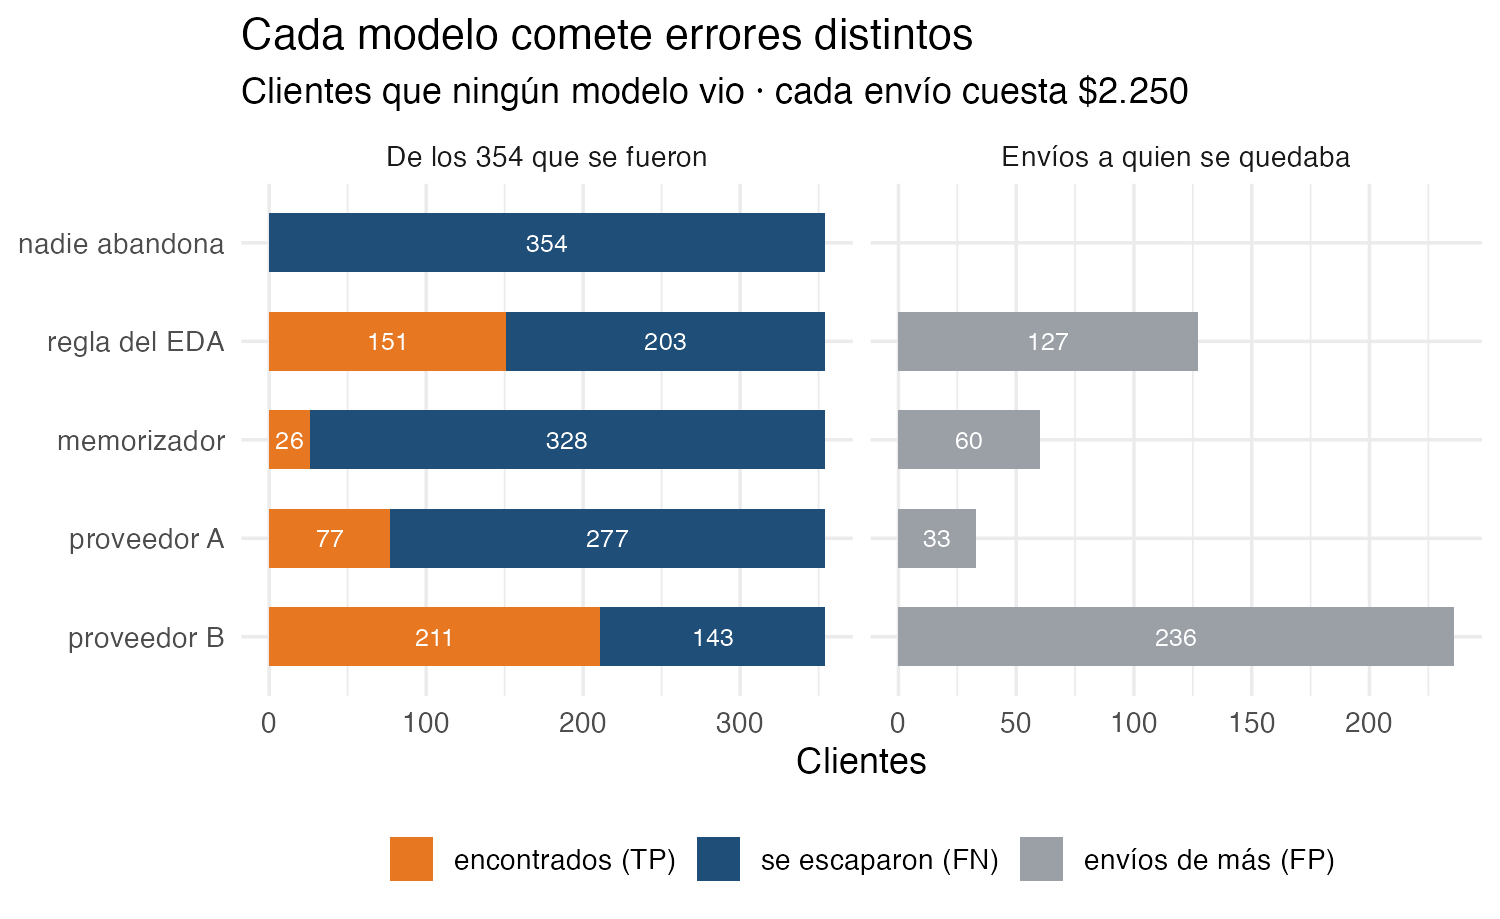
\includegraphics[width=0.8\textwidth]{pic/fig_tipos_error_s10.png}
\end{center}
\vspace{-0.15cm}
\footnotesize
El proveedor A casi no envía de más, pero se le escapan 277 de 354. El B encuentra 211, a cambio de 236 envíos innecesarios. El memorizador encuentra apenas 26.
\end{frame}

%%=================================================
\begin{frame}{Tres métricas, tres preguntas}
\small
\begin{columns}[T]
\column{0.55\textwidth}
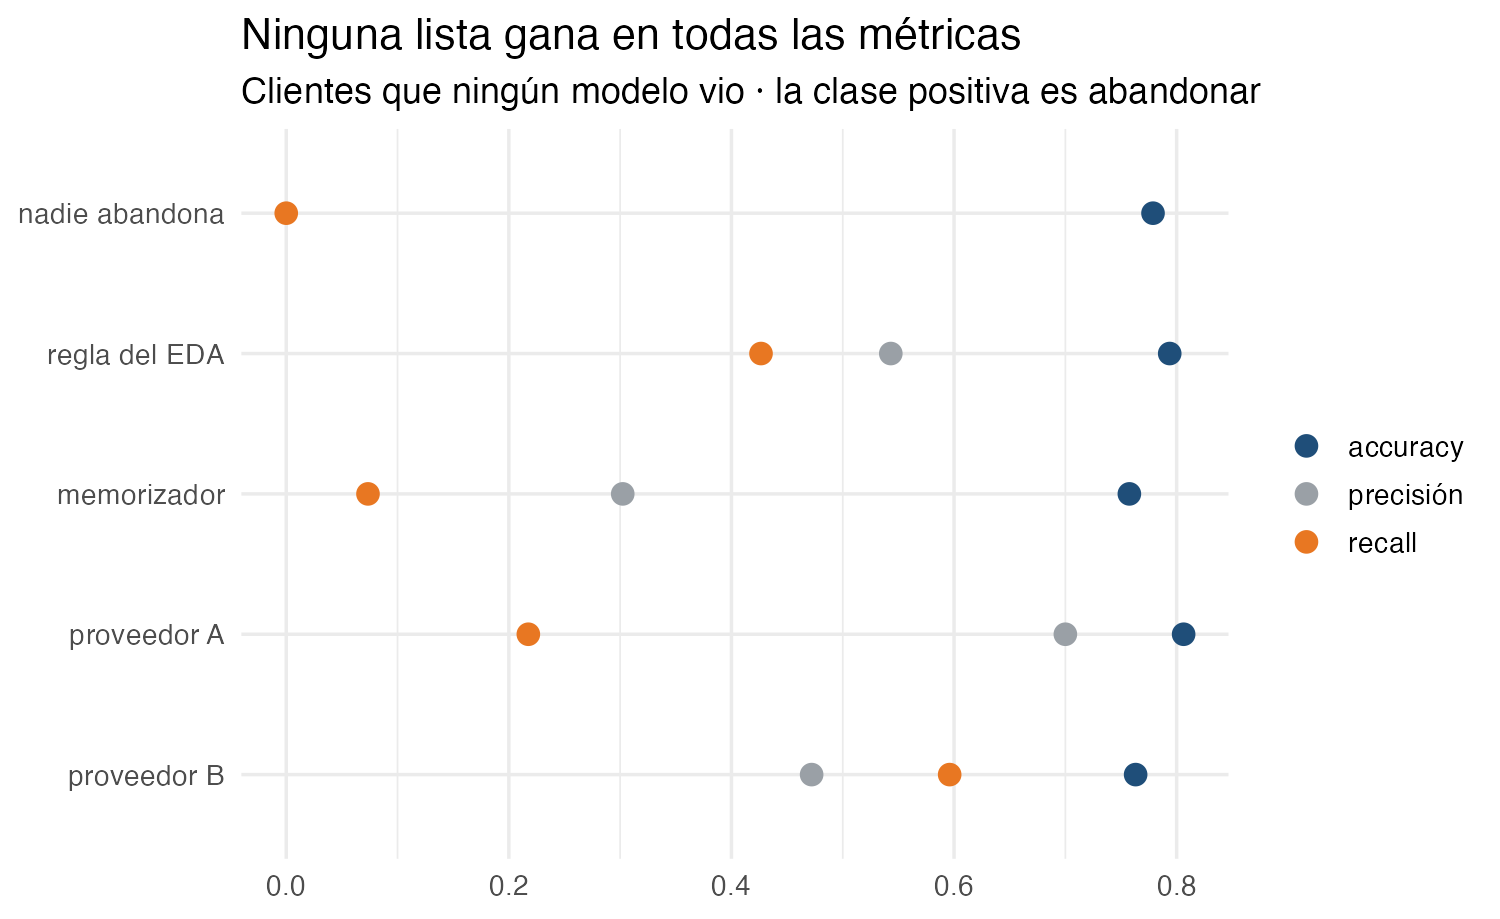
\includegraphics[width=\textwidth]{pic/fig_metricas_s10.png}
\column{0.43\textwidth}
\footnotesize
\begin{itemize} \setlength{\itemsep}{0.14cm}
  \item \textbf{Accuracy}: ¿qué fracción de los clientes clasificó bien? Gana A (0.806)\ldots\ pero no hacer nada ya logra 0.779.
  \item \textbf{Precisión}: de los que reciben la campaña, ¿cuántos se iban? Gana A (0.700).
  \item \textbf{Recall}: de los que se iban, ¿a cuántos encontró? Gana B (0.596).
\end{itemize}
\end{columns}
\vspace{0.15cm}
\begin{alertblock}{Lo que importa}
Cada métrica premia a un modelo distinto. Antes de elegir, hay que decidir qué pregunta le importa a Growth.
\end{alertblock}
\end{frame}

%%=================================================
\begin{frame}{¿Cuánto cuesta cada lista y a cuántos encuentra?}
\small
\begin{columns}[T]
\column{0.52\textwidth}
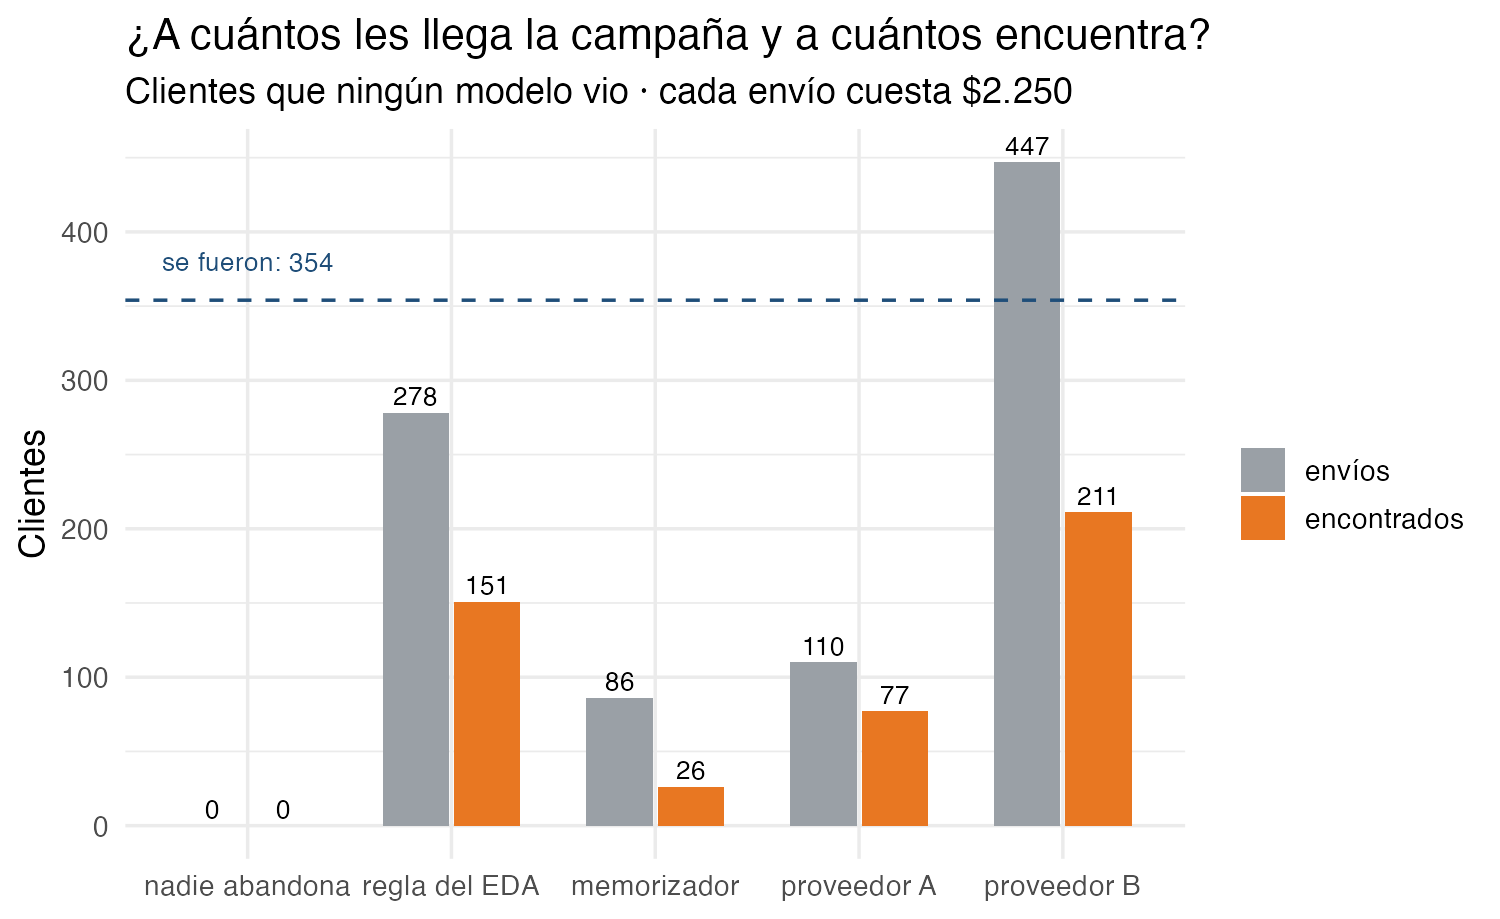
\includegraphics[width=\textwidth]{pic/fig_envios_s10.png}
\column{0.46\textwidth}
\centering
\scriptsize
\setlength{\tabcolsep}{2.5pt}
\begin{tabular}{@{}l r c r@{}}
\toprule
\textbf{Modelo} & \textbf{Costo} & \textbf{Encontr.} & \textbf{Por enc.} \\
\midrule
Prov. A & \$247.500 & 77 & \$3.214 \\
Regla & \$625.500 & 151 & \$4.142 \\
Prov. B & \$1.005.750 & 211 & \$4.767 \\
Memoriz. & \$193.500 & 26 & \$7.442 \\
\bottomrule
\end{tabular}

\vspace{0.1cm}
\raggedright
\footnotesize
Costo = envíos $\times$ \$2.250.
\end{columns}
\vspace{0.15cm}
\begin{alertblock}{Lo que importa}
Encontrar más clientes cuesta más, y no todos los envíos rinden igual: el memorizador paga más del doble por cada cliente que el proveedor A.
\end{alertblock}
\end{frame}

%%=================================================
\begin{frame}{¿Cuánto cuesta encontrar un cliente más?}
\small
\begin{columns}[T]
\column{0.55\textwidth}
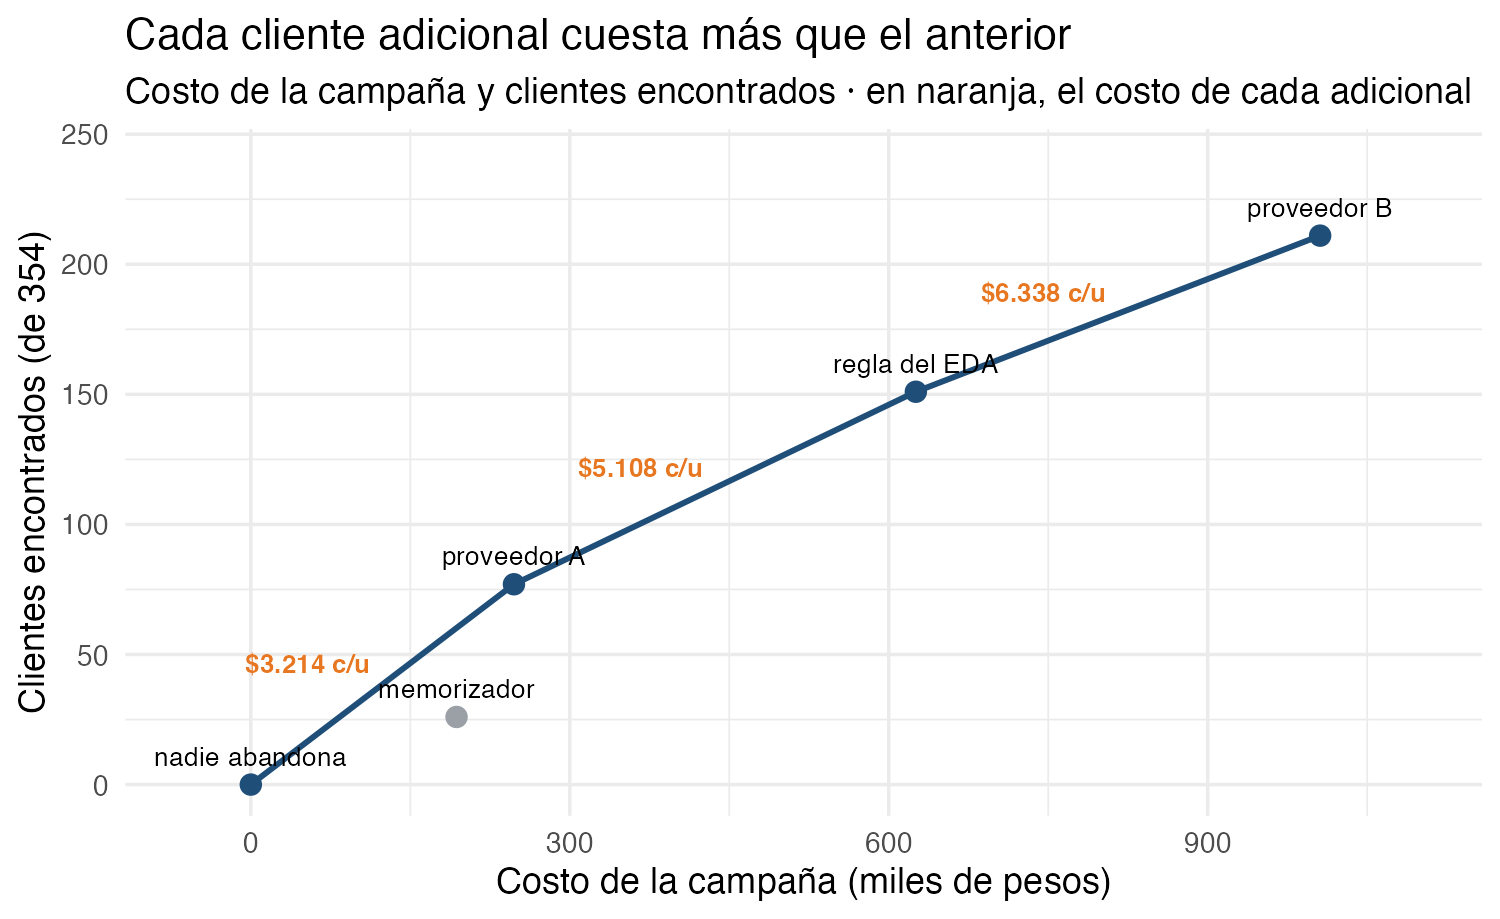
\includegraphics[width=\textwidth]{pic/fig_frontera_s10.png}
\column{0.43\textwidth}
\footnotesize
\begin{itemize} \setlength{\itemsep}{0.12cm}
  \item De no enviar nada al proveedor A: \textbf{\$3.214} por cliente encontrado.
  \item Del proveedor A a la regla: \textbf{\$5.108} por cada uno de los 74 adicionales.
  \item De la regla al proveedor B: \textbf{\$6.338} por cada uno de los 60 adicionales.
  \item El memorizador queda por debajo de la línea: con 24 envíos más, el proveedor A encuentra 51 clientes más.
\end{itemize}
\end{columns}
\vspace{0.15cm}
\begin{alertblock}{Lo que importa}
Ampliar la lista conviene mientras cada cliente adicional valga más de lo que cuesta encontrarlo.
\end{alertblock}
\end{frame}

%%=================================================
\begin{frame}{La recomendación: ¿cuánto vale encontrar a un cliente?}
\small
Encontrar a un cliente no es retenerlo. Cada cliente encontrado vale \textbf{la fracción que la campaña retiene} $\times$ \textbf{lo que deja un cliente retenido}. Con \$40.000 por cliente retenido (cifras ilustrativas):

\vspace{0.1cm}
\begin{center}
\scriptsize
\setlength{\tabcolsep}{6pt}
\begin{tabular}{@{}l r r@{}}
\toprule
\textbf{Beneficio neto} & \textbf{Retiene 1 de cada 10} & \textbf{Retiene 2 de cada 10} \\
\textit{(encontrados $\times$ valor $-$ costo)} & \textit{cada uno vale \$4.000} & \textit{cada uno vale \$8.000} \\
\midrule
Proveedor A & \textbf{\$60.500} & \$368.500 \\
Regla del EDA & $-$\$21.500 & \$582.500 \\
Proveedor B & $-$\$161.750 & \textbf{\$682.250} \\
Memorizador & $-$\$89.500 & \$14.500 \\
No enviar a nadie & \$0 & \$0 \\
\bottomrule
\end{tabular}
\end{center}
\pause
\begin{alertblock}{La recomendación}
Con \$4.000 por cliente, solo paga el primer tramo (\$3.214 hasta el proveedor A): conviene \textbf{A}. Con \$8.000, pagan todos los tramos (hasta \$6.338): conviene \textbf{B}. Los modelos no cambiaron; cambió cuánto vale cada acierto.
\end{alertblock}
\end{frame}

%%=================================================
\section{Finanzas: ¿cuánto gastará cada cliente?}

\begin{frame}{¿Qué cambia cuando predecimos un monto y no una categoría?}
\small
Finanzas quiere saber cuánto gastará cada cliente el próximo trimestre. Ya no hay acierto o error: hay una \textbf{distancia}, en pesos.

\vspace{0.1cm}
\begin{columns}[T]
\column{0.42\textwidth}
\centering
\scriptsize
\setlength{\tabcolsep}{4pt}
\begin{tabular}{@{}c r r r@{}}
\toprule
\textbf{Cliente} & \textbf{Real} & \textbf{Pronóstico} & \textbf{Error} \\
\midrule
1 & 120 & 120 & 0 \\
2 & 80 & 90 & 10 \\
3 & 200 & 190 & 10 \\
4 & 150 & 120 & 30 \\
\rowcolor{grisclaro} 5 & 400 & 270 & \textbf{130} \\
\bottomrule
\end{tabular}

\vspace{0.05cm}
\tiny Ilustrativo, en miles de pesos.
\column{0.55\textwidth}
\footnotesize
\begin{itemize} \setlength{\itemsep}{0.14cm}
  \item \textbf{MAE}, el error típico: el promedio de los errores. El de 0, 10, 10, 30 y 130 es \textbf{36 mil}.
  \item \textbf{RMSE}, que castiga los errores grandes: se elevan al cuadrado (0, 100, 100, 900 y 16.900), se promedian (3.600) y se saca la raíz: \textbf{60 mil}.
\end{itemize}
\end{columns}
\vspace{0.15cm}
\begin{alertblock}{Lo que importa}
Un solo cliente con un error grande hace que el RMSE casi duplique al MAE.
\end{alertblock}
\end{frame}

%%=================================================
\begin{frame}{¿Qué pronóstico le sirve a Finanzas?}
\small
\begin{columns}[T]
\column{0.52\textwidth}
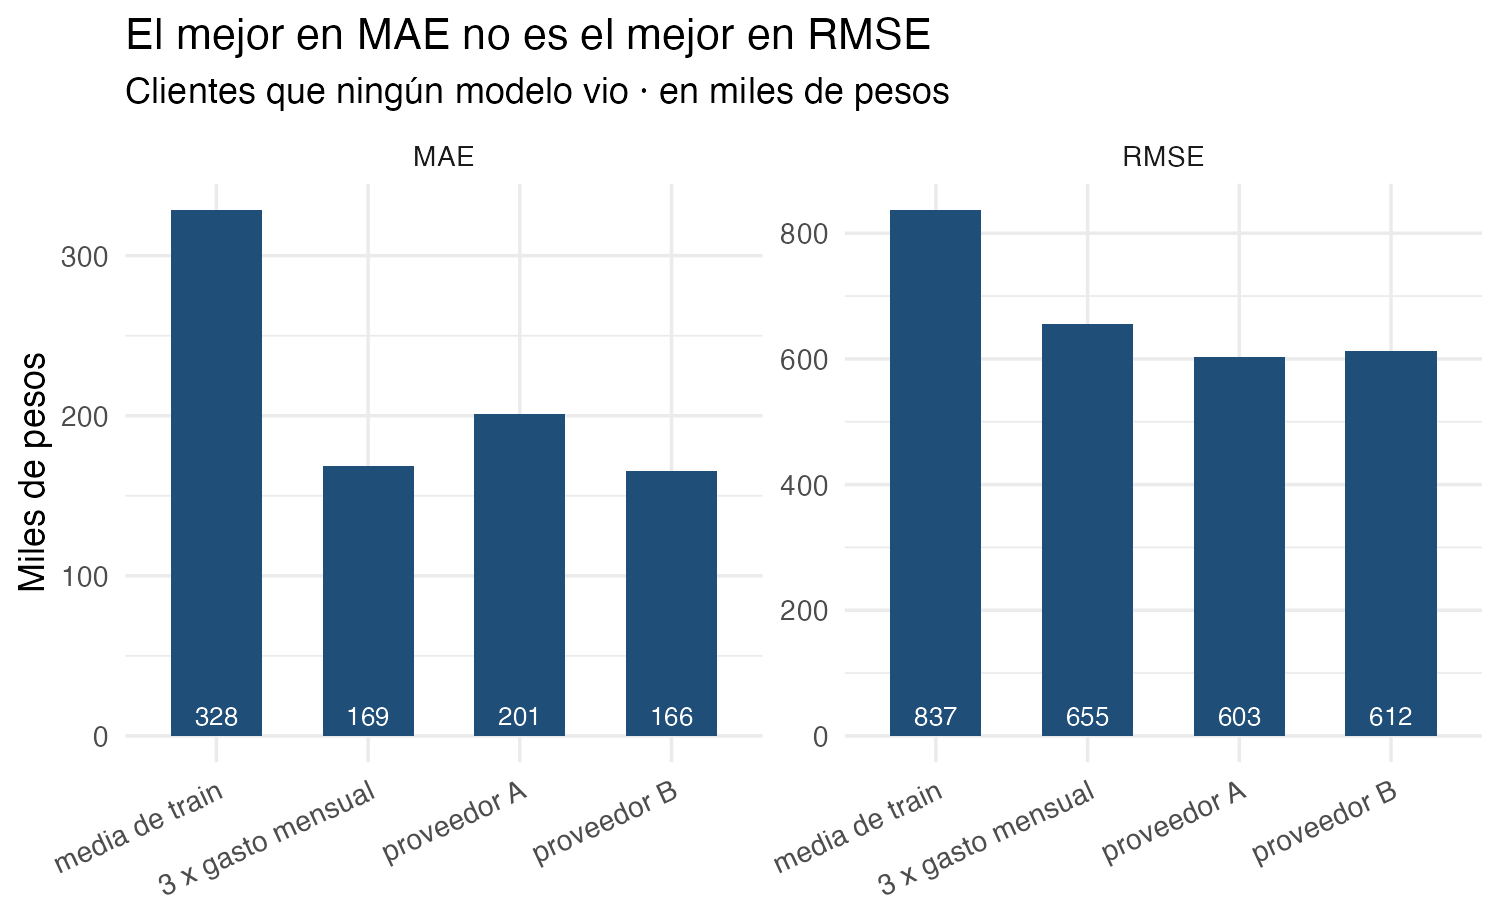
\includegraphics[width=\textwidth]{pic/fig_errores_s10.png}
\column{0.46\textwidth}
\footnotesize
\begin{itemize} \setlength{\itemsep}{0.12cm}
  \item Los tres le ganan a la media (MAE 328.494).
  \item \textbf{Regla} y \textbf{proveedor B}: casi el mismo MAE (168.728 y 165.540); B comete errores grandes menores (RMSE 612.315 frente a 655.018).
  \item \textbf{Proveedor A}: el mejor RMSE (602.617), pero el peor MAE de los tres y \textcolor{rojoal}{413 pronósticos negativos}.
\end{itemize}
\end{columns}
\pause
\vspace{0.1cm}
\begin{alertblock}{La recomendación}
Si importa el error típico, la regla y B empatan; si cuestan los errores grandes, conviene B. A se descarta: un gasto negativo es imposible.
\end{alertblock}
\end{frame}

%%=================================================
\section{Lo que nos llevamos}

\begin{frame}{Lo que nos llevamos}
\small
\begin{block}{La idea de hoy}
Una métrica por sí sola no escoge el modelo: la elección depende de la pregunta y del costo de equivocarse.
\end{block}

\vspace{0.1cm}
\begin{itemize} \setlength{\itemsep}{0.14cm}
  \item \textbf{Growth}: el que más acierta (A) no es el que más clientes encuentra (B). Cuál conviene depende de cuánto vale retener a un cliente.
  \item \textbf{Finanzas}: el mejor en MAE no es el mejor en RMSE. Depende de cuánto cuestan los errores grandes.
\end{itemize}

\vspace{0.1cm}
\footnotesize
\textbf{Ahora}, con el monitor: corran \texttt{10\_juez\_condor.R}, que sigue esta misma secuencia con sus propias salidas. \textbf{El taller} está al final del script (su escenario para Growth y su pronóstico para Finanzas) y se sube a Intu antes de terminar la clase. \textbf{La semana 11}: Cóndor construye sus propios modelos.
\end{frame}

%%=================================================
\appendix
\begin{frame}[noframenumbering]{Apéndice · ¿Y el AUC?}
\small
\begin{columns}[T]
\column{0.55\textwidth}
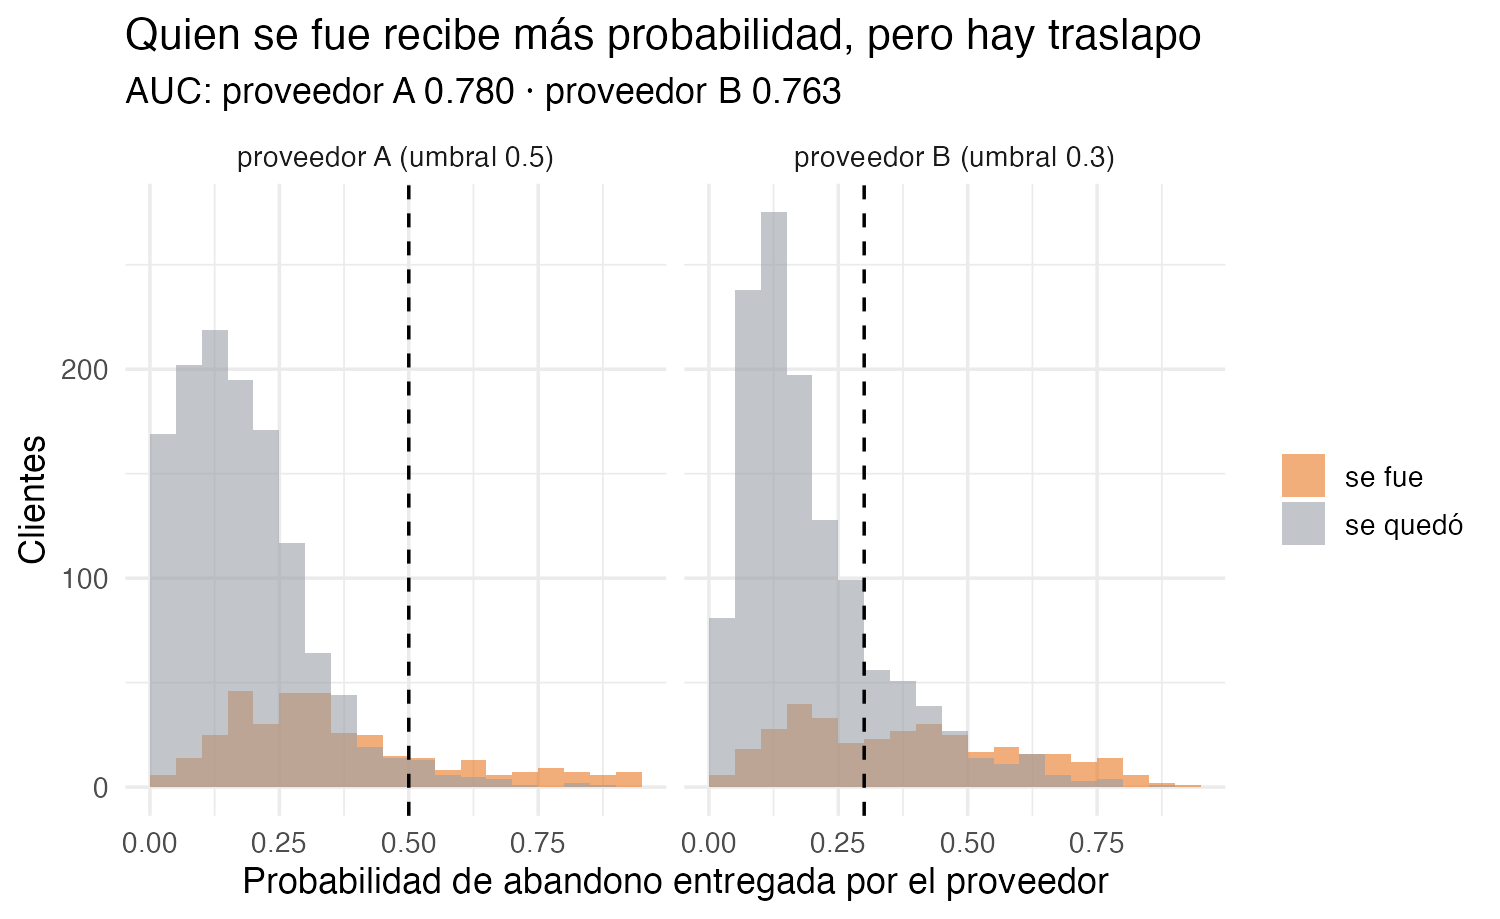
\includegraphics[width=\textwidth]{pic/fig_probabilidades_s10.png}
\column{0.43\textwidth}
\footnotesize
Los proveedores también entregan una probabilidad por cliente. El AUC responde: si tomo a uno que se fue y a uno que se quedó, \textbf{¿con qué frecuencia el modelo le da más probabilidad al que se fue?}

\vspace{0.12cm}
A: \textbf{0.780}; B: \textbf{0.763}. Ordenar al azar daría 0.5.

\vspace{0.12cm}
Hoy no cambia la decisión: Growth recibe listas ya armadas, y las listas se evalúan por lo que encuentran y lo que cuestan.
\end{columns}
\end{frame}

\end{document}
